This appendix provides additional experimental details along with qualitative and quantitative results.
Additionally, we discuss our diffusion-based baseline and \leffa{} loss, along with their limitations.

\section{Experimental Details}

\subsection{Datasets}
In this section, we provide a detailed introduction to the three datasets used in our study.

\noindent \textbf{VITON-HD}~\citep{choi2021viton} dataset is the most commonly used dataset for virtual try-on task.
The training set contains 11,647 person and garment image pairs, and the test set contains 2,032 pairs.
All images are front-view, upper-body garments with a resolution of $1024 \times 768$.

\noindent \textbf{DressCode}~\citep{morelli2022dress} dataset is composed of various types of garments, comprising 48,392 person and garment image pairs in the training set.
This includes 13,563 upper-body, 7,151 lower-body, and 27,678 dress garment pairs.
The test set contains 5,400 pairs, evenly distributed across 1,800 pairs each for upper-body, lower-body, and dress garments.
All images have a resolution of $1024 \times 768$.

\noindent \textbf{DeepFashion}~\citep{liu2016deepfashion} dataset includes high resolution 52,712 person images in the fashion domain.
Following ~\citet{zhu2019progressive}, we split the dataset into training and test subsets with 101,966 and 8,570 pairs, respectively.
Each pair includes the same person in the same garment but with different poses.


\section{More Results for DressCode Dataset}

To further validate our performance, we conduct separate evaluations on different garment categories for the DressCode dataset.
In Tab.~\ref{leffa:tab:dresscode_v2}, results show that our method significantly outperforms previous methods across all garment categories.
Specifically, for the upper body category, it achieves an FID reductions of -2.33 (paired) and -0.91 (unpaired); for the lower body category, -2.94 (paired) and -2.55 (unpaired); and for dresses, -1.25 (paired) and -1.71 (unpaired).

\begin{table}[!t]
\centering
\setlength{\tabcolsep}{0.2cm}
\caption{Quantitative results comparison with other methods on the DressCode dataset for virtual try-on.
Our \leffa{} achieves state-of-the-art results across all categories of garment.
}
\resizebox{0.88\linewidth}{!}{
\begin{tabular}{lcccccc}
\toprule[1.5pt]
\multirow{2}{*}{\textbf{Method}}        & \multicolumn{4}{c}{\textbf{paired}} & \multicolumn{2}{c}{\textbf{unpaired}} \\ \cmidrule{2-7} 
                                        & \textbf{FID} $\downarrow$ & \textbf{KID} $\downarrow$ & \textbf{SSIM} $\uparrow$ & \textbf{LPIPS} $\downarrow$ & \textbf{FID} $\downarrow$ & \textbf{KID} $\downarrow$ \\ \midrule
\rowcolor{tablegray} \multicolumn{7}{c}{upper body} \\
FS-VTON~\citep{he2022style}             & 11.29 & 3.65 & 0.941 & \underline{0.035} & 16.34 & 5.93 \\
HR-VITON~\citep{lee2022high}            & 15.36 & 5.27 & 0.916 & 0.071 & 16.82 & 5.70 \\
GP-VTON~\citep{xie2023gp}               & \underline{7.38}  & 0.74 & \underline{0.945} & 0.039 & 12.21 & 1.19 \\
LADI-VTON~\citep{morelli2023ladi}       & 9.53  & \underline{0.20} & 0.928 & 0.049 & 13.26 & 2.67 \\
DCI-VTON~\citep{gou2023taming}          & 7.47  & 1.07 & 0.942 & 0.041 & \underline{11.64} & \underline{0.86} \\
StableVITON~\citep{kim2024stableviton}  & 9.94  & 0.12 & 0.937 & 0.039 & -     & -    \\
OOTDiffusion~\citep{xu2024ootdiffusion} & 11.03 & 0.29 & -     & -     & -     & -    \\
% $D^{4}$-VTON~\citep{yang2024d}          & 6.55  & 0.23 & 0.946 & 0.032 & 10.99 & 0.30 \\
\textbf{\leffa{} (Ours)}                 & \textbf{5.05}  & \textbf{0.02} & \textbf{0.949} & \textbf{0.021} & \textbf{10.73} & \textbf{0.77} \\
\rowcolor{tablegray} \multicolumn{7}{c}{lower body} \\
FS-VTON~\citep{he2022style}             & 11.65 & 3.82 & 0.934 & 0.053 & 22.43 & 9.81 \\
HR-VITON~\citep{lee2022high}            & 11.41 & 3.20 & 0.937 & 0.045 & 16.39 & 4.31 \\
GP-VTON~\citep{xie2023gp}               & \underline{7.73}  & \underline{0.71} & 0.938 & \underline{0.042} & 16.70 & 2.89 \\
LADI-VTON~\citep{morelli2023ladi}       & 8.52  & 1.04 & 0.922 & 0.051 & \underline{14.80} & 3.13 \\
DCI-VTON~\citep{gou2023taming}          & 7.97  & 0.96 & \underline{0.939} & 0.045 & 15.45 & \underline{1.60} \\
% $D^{4}$-VTON~\citep{yang2024d}          & 6.68  & 0.04 & 0.946 & 0.033 & 14.86 & 1.50 \\
\textbf{\leffa{} (Ours)}                 & \textbf{4.79}  & \textbf{0.05} & \textbf{0.941} & \textbf{0.024} & \textbf{12.25} & \textbf{1.66} \\
\rowcolor{tablegray} \multicolumn{7}{c}{dresses} \\
FS-VTON~\citep{he2022style}             & 13.04 & 4.44 & \underline{0.888} & \underline{0.070} & 20.95 & 8.96 \\
HR-VITON~\citep{lee2022high}            & 16.82 & 4.89 & 0.865 & 0.113 & 18.81 & 5.41 \\
GP-VTON~\citep{xie2023gp}               & \underline{7.44}  & \textbf{0.32} & 0.881 & 0.073 & 12.64 & 1.83 \\
LADI-VTON~\citep{morelli2023ladi}       & 9.07  & 1.12 & 0.868 & 0.089 & 13.40 & 2.50 \\
DCI-VTON~\citep{gou2023taming}          & 8.48  & \underline{1.08} & 0.887 & \underline{0.070} & \underline{12.35} & \underline{1.36} \\
% $D^{4}$-VTON~\citep{yang2024d}          & 8.28  & 1.07 & 0.890 & 0.061 & 12.29 & 1.14 \\
\textbf{\leffa{} (Ours)}                 & \textbf{6.19}  & \textbf{0.32} & \textbf{0.891} & \textbf{0.044} & \textbf{10.64} & \textbf{0.59} \\
\bottomrule[1.5pt]
\end{tabular}
}
\label{leffa:tab:dresscode_v2}
\end{table}



\begin{table}[!t]
\centering
\setlength{\tabcolsep}{0.2cm}
\caption{Ablation study on DressCode dataset for virtual try-on.
Our \leffa{} loss significantly improves model performance.
}
\resizebox{0.88\linewidth}{!}{
\begin{tabular}{lccccccc}
\toprule[1.5pt]
\multirow{2}{*}{\textbf{Method}}  & \multirow{2}{*}{\textbf{$\mathcal{L}_{\text{leffa}}$}}        & \multicolumn{4}{c}{\textbf{paired}} & \multicolumn{2}{c}{\textbf{unpaired}} \\ \cmidrule{3-8} 
                                        & & \textbf{FID} $\downarrow$ & \textbf{KID} $\downarrow$ & \textbf{SSIM} $\uparrow$ & \textbf{LPIPS} $\downarrow$ & \textbf{FID} $\downarrow$ & \textbf{KID} $\downarrow$ \\ 
\midrule
\multirow{2}{*}{Ours}   & \xmark & 3.64  & 0.33 & 0.911 & 0.040 & 5.98  & 1.42 \\
                        & \cmark & \textbf{2.06}  & \textbf{0.07} & \textbf{0.924} & \textbf{0.031} & \textbf{4.48}  & \textbf{0.62} \\
\bottomrule[1.5pt]
\end{tabular}
}
\label{leffa:tab:ablation_dress_code}
\end{table}


\begin{table}[!t]
\centering
\setlength{\tabcolsep}{0.5cm}
\caption{Ablation study on the DeepFashion dataset for pose transfer.
Our \leffa{} loss significantly improves model performance.
}
\resizebox{0.8\linewidth}{!}{
\begin{tabular}{lcccc}
\toprule[1.5pt]
\textbf{Method} & \textbf{$\mathcal{L}_\text{leffa}$} & \textbf{FID} $\downarrow$ & \textbf{SSIM} $\uparrow$ & \textbf{LPIPS} $\downarrow$ \\
\midrule
\multirow{2}{*}{Ours ($512 \times 352$)} & \xmark & 5.72 & 0.744 & 0.153 \\
                                    & \cmark & \textbf{4.23}  & \textbf{0.755} & \textbf{0.119} \\
\bottomrule[1.5pt]
\end{tabular}
}
\label{leffa:tab:ablation_deep_fashion}
\end{table}



\section{More Ablation Studies}
Unless stated otherwise, the ablation studies are conducted on the VITON-HD dataset for the virtual try-on task, in alignment with Chapter~6.

\noindent \textbf{Effect of $\mathcal{L}_\text{leffa}$}.
To validate the effectiveness of \leffa{} loss, we conduct ablation studies on the DressCode dataset for virtual try-on and the DeepFashion dataset for pose transfer.
i) As shown in Tab.~\ref{leffa:tab:ablation_dress_code}, our \leffa{} reduces FID by -1.58 in the paired setting and -1.5 in the unpaired setting.
ii) Tab.~\ref{leffa:tab:ablation_deep_fashion} further shows an FID reduction of -1.49 on pose transfer task.
These results confirm that \leffa{} loss significantly improves controllable person image generation, enhancing both appearance and pose control.

% \noindent \textbf{Qualitative Impact of Our \leffa{} Loss $\mathcal{L}_\text{leffa}$}.
% In Fig.~\ref{leffa:fig:vis_ablation_v2}, we visualize attention maps with varying $\lambda_\text{leffa}$ to assess its impact on model training.
% The first row shows generated results with different $\lambda_{\text{leffa}}$ values, with $\lambda_{\text{leffa}} = 0$ indicating no $\mathcal{L}_{\text{leffa}}$.
% Rows 2 to 5 highlight reference key regions attended by the target query, marked by arrows of various colors.
% Without $\mathcal{L}{\text{leffa}}$, attention is dispersed.
% Increasing $\lambda_{\text{leffa}}$ improves focus, guiding the query to correct regions.
% However, when $\lambda_{\text{leffa}} > 10^{-3}$, the attention becomes overly narrow and less accurate, hindering image generation.


% \begin{figure*}[t]
%     \centering
%     % \fbox{\rule{0pt}{2in} \rule{1.0\linewidth}{0pt}}
%     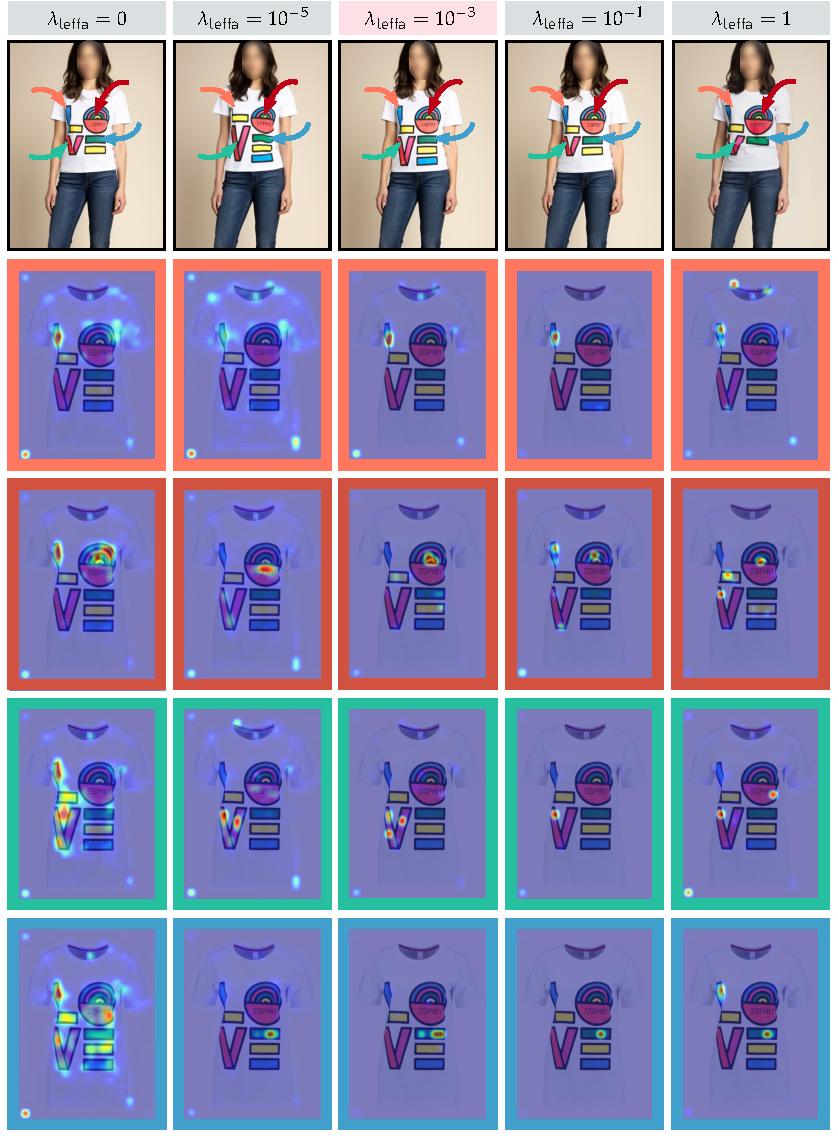
\includegraphics[width=0.95\linewidth]{Chapter6/Figures/vis_ablation_v2_final.pdf}
%     \caption{
%     More visualizations of feature maps to assess the impact of \leffa{} loss.
%     The third column is the optimal setting used in this chapter.
%     }
%     \label{leffa:fig:vis_ablation_v2}
% \end{figure*}


\noindent \textbf{Effect of Averaging Attention Map Across Multi-Head}.
Inspired by~\cite{darcet2023vision}, we average the attention maps across all heads before computing the \leffa{} loss.
As shown in Tab.~\ref{leffa:tab:more_ablation} (\leffa{} w/o average $A$), computing the loss for each head individually degrades performance, emphasizing the role of redundancy in attention maps for better generalization.

\noindent \textbf{Effect of Upsampling Flow Fields}.
To evaluate the impact of upsampling the flow fields to image resolution, we experiment with retaining their latent resolution for the \leffa{}, requiring the ground truth image to be downsampled.
This resizing reduces detail, hindering accurate supervision.
As shown in Tab.~\ref{leffa:tab:more_ablation} (\leffa{} w/o upsample $\mathcal{F}$), not upsampling the flow fields results in a performance drop, further supporting our viewpoint.


\begin{table}[!t]
\centering
\setlength{\tabcolsep}{0.2cm}
\caption{Ablation study for the proposed \leffa{} loss.}
\resizebox{0.84\linewidth}{!}{
\begin{tabular}{lcccccc}
\toprule[1.5pt]
\multirow{2}{*}{\textbf{Method}}        & \multicolumn{4}{c}{\textbf{paired}} & \multicolumn{2}{c}{\textbf{unpaired}} \\ \cmidrule{2-7} 
                                        & \textbf{FID} $\downarrow$ & \textbf{KID} $\downarrow$ & \textbf{SSIM} $\uparrow$ & \textbf{LPIPS} $\downarrow$ & \textbf{FID} $\downarrow$ & \textbf{KID} $\downarrow$ \\ \midrule
\leffa{} (Ours)                          & \textbf{4.54}  & \textbf{0.05} & \textbf{0.899} & \textbf{0.048} & \textbf{8.52}  & \textbf{0.32} \\
\leffa{} w/o average $A$                 & 6.02 & 0.74 & 0.863 & 0.072 & 9.78 & 0.98 \\
\leffa{} w/o upsample $\mathcal{F}$      & 4.94 & 0.32 & 0.888 & 0.064 & 9.33 & 0.78 \\
\bottomrule[1.5pt]
\end{tabular}
}
\label{leffa:tab:more_ablation}
\end{table}



\section{Discussion}
\label{leffa:sec:discussion}

\noindent \textbf{Why Does Our Diffusion-Based Baseline Perform Comparably to State-of-the-Art Methods?}
Our baseline is similar to existing virtual try-on and pose transfer methods~\citep{choi2024improving, xu2024ootdiffusion, bhunia2023person, han2023controllable}, but we find that complex designs are unnecessary for strong performance.
The key lies in making both UNets in the dual architecture fully trainable, as freezing one significantly degrades results.
As shown in Tab.~\ref{leffa:tab:ablation_baseline}, freezing the reference UNet (as done in \citet{choi2024improving}) leads to a significant performance drop (FID reduction of -1.11/-1.25 for the paired/unpaired settings).
In contrast, adding CLIP visual and textual features~\citep{choi2024improving, xu2024ootdiffusion} results in only a slight performance decline.
This highlights that the key to improving the baseline lies in making both UNets trainable, while adding more complex designs (\eg, add CLIP, textual information) is unnecessary.


\begin{table}[!t]
\centering
\setlength{\tabcolsep}{0.2cm}
\caption{Ablation study for our diffusion-based baseline.
Making both the generative and reference UNets trainable is key to performance improvement for our diffusion-based baseline.
}
\resizebox{0.84\linewidth}{!}{
\begin{tabular}{lcccccc}
\toprule[1.5pt]
\multirow{2}{*}{\textbf{Method}}        & \multicolumn{4}{c}{\textbf{paired}} & \multicolumn{2}{c}{\textbf{unpaired}} \\ \cmidrule{2-7} 
                                        & \textbf{FID} $\downarrow$ & \textbf{KID} $\downarrow$ & \textbf{SSIM} $\uparrow$ & \textbf{LPIPS} $\downarrow$ & \textbf{FID} $\downarrow$ & \textbf{KID} $\downarrow$ \\ \midrule
Our baseline                & \textbf{5.31} & \textbf{0.30} & 0.885 & 0.058 & \textbf{9.38} & \textbf{0.91} \\
freeze Reference UNet       & 6.42 & 0.77 & 0.863 & 0.066 & 10.63 & 1.32 \\
+ CLIP visual feature       & 5.33 & 0.31 & \textbf{0.886} & \textbf{0.056} & 9.40 & 0.95 \\
+ CLIP textual feature      & 5.37 & 0.40 & 0.876 & 0.060 & 9.45 & 0.98 \\
\bottomrule[1.5pt]
\end{tabular}
}
\label{leffa:tab:ablation_baseline}
\end{table}


\noindent \textbf{Why Not Add $\mathcal{L}_{\text{leffa}}$ from the First Training Stage?}
At the start of training, the attention maps are not well learned, and applying our \leffa{} loss too early forces the target query to prematurely attend to the reference key, hindering convergence rather than accelerating it.
Instead, introducing our \leffa{} loss in a subsequent training stage significantly enhances performance, demonstrating its ability to correct inaccurate attention and guide the model toward more effective learning.


\section{Limitations}
While \leffa{} significantly improves controllable person image generation in appearance and pose control, it has several limitations. 
First, it requires multi-stage training with the \leffa{} loss applied only in the final stage.
In future work, we aim to design a single-stage model to simplify the training process.
% Suggest to add something like: \leffa{} also encounters challenges commonly associated with using off-the-shelf backbones. For example, 
Second, appearance control relies on garment segmentation, which impacts performance when segmentation is inaccurate.
We plan to develop a mask-free approach to ensure high quality generation and preserve fine-grained details without distortion.
Third, our method struggles to preserve extremely fine-grained details, such as small text, due to the $8\times$ resolution compression brought by the latent encoder in the latent diffusion model.
% \brandon{We should clarify the 2 and 3 are the common issues, not our specific limitations.}
It is worth noting that the issues mentioned above are not unique to our method but are also present in other methods.


% \section{More Qualitative Comparison}
% To further demonstrate the effectiveness of our \leffa{}, we conduct qualitative comparisons with other methods on the VITON-HD, DressCode, and DeepFashion datasets, as shown in Figs.~\ref{leffa:fig:supp_vis_1}--\ref{leffa:fig:supp_vis_6}.
% The results indicate that our \leffa{} not only generates images with higher overall quality but also significantly alleviates fine-grained detail distortion.


% \begin{figure*}[t]
%     \centering
%     % \fbox{\rule{0pt}{2in} \rule{1.0\linewidth}{0pt}}
%     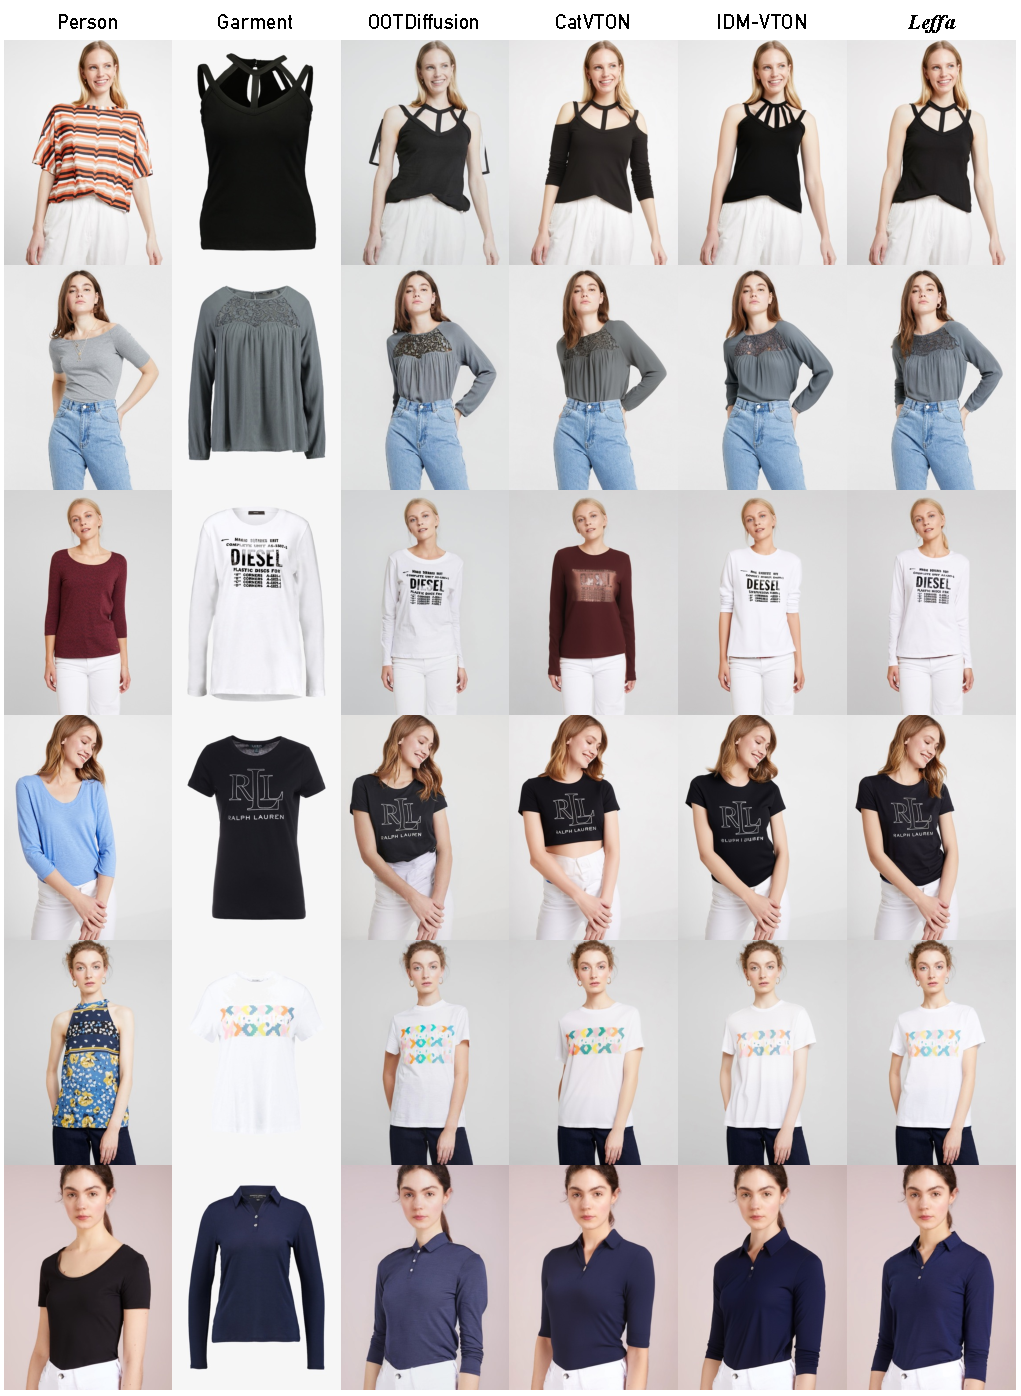
\includegraphics[width=0.95\linewidth]{Chapter6/Figures/supp_1.pdf}
%     \caption{
%     Qualitative visual results comparison with other methods on VITON-HD for virtual try-on (Part 1).
%     }
%     \label{leffa:fig:supp_vis_1}
% \end{figure*}

% \begin{figure*}[t]
%     \centering
%     % \fbox{\rule{0pt}{2in} \rule{1.0\linewidth}{0pt}}
%     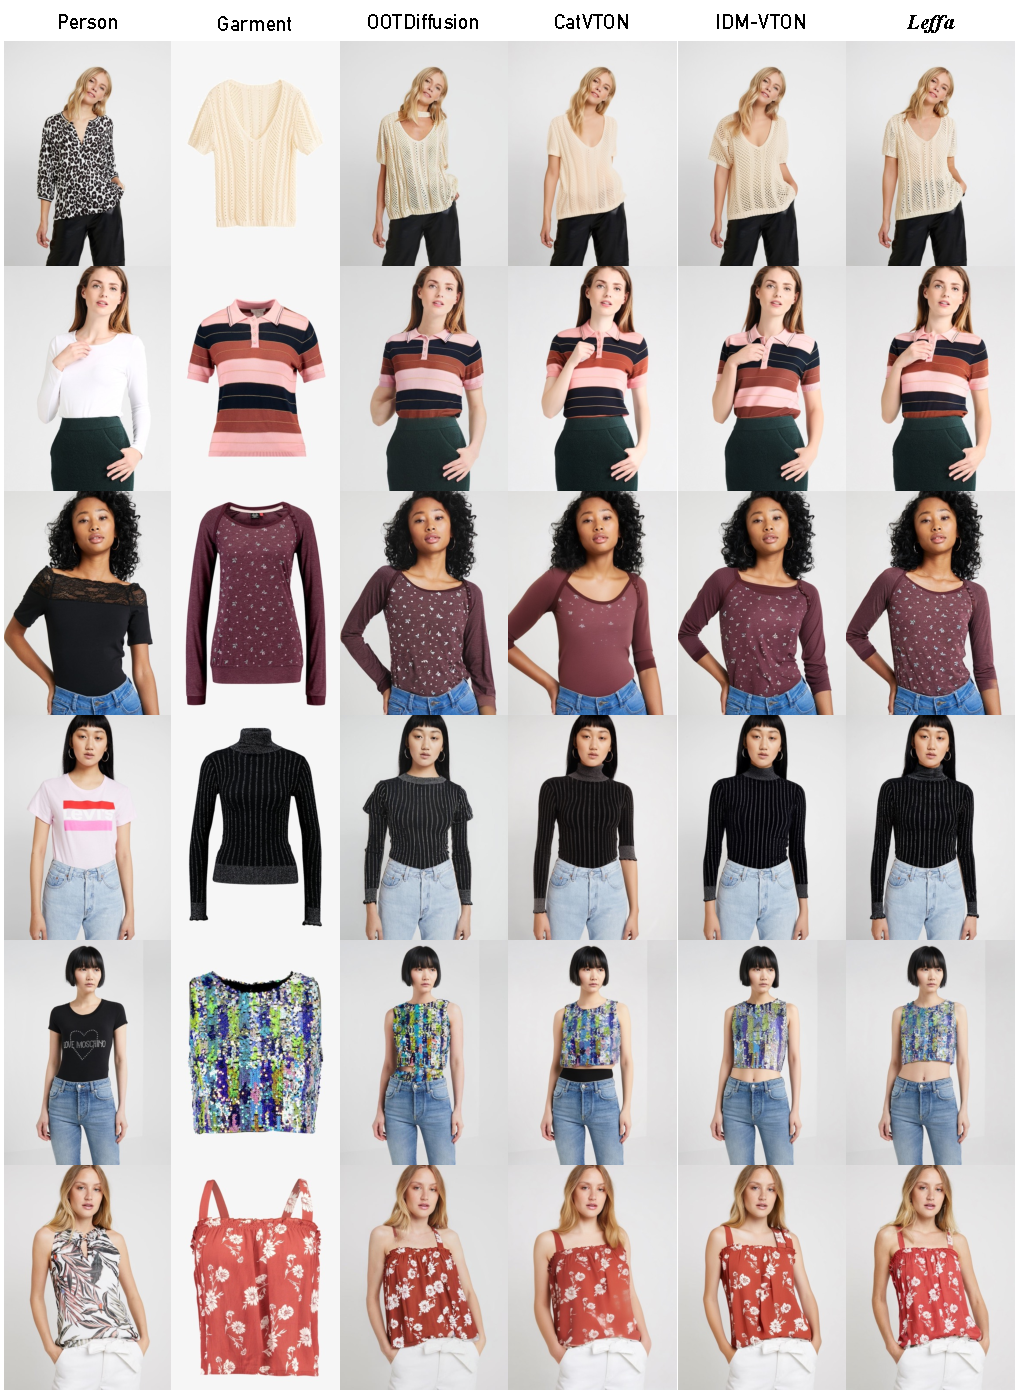
\includegraphics[width=0.95\linewidth]{Chapter6/Figures/supp_2.pdf}
%     \caption{
%     Qualitative visual results comparison with other methods on VITON-HD for virtual try-on (Part 2).
%     }
%     \label{leffa:fig:supp_vis_2}
% \end{figure*}

% \begin{figure*}[t]
%     \centering
%     % \fbox{\rule{0pt}{2in} \rule{1.0\linewidth}{0pt}}
%     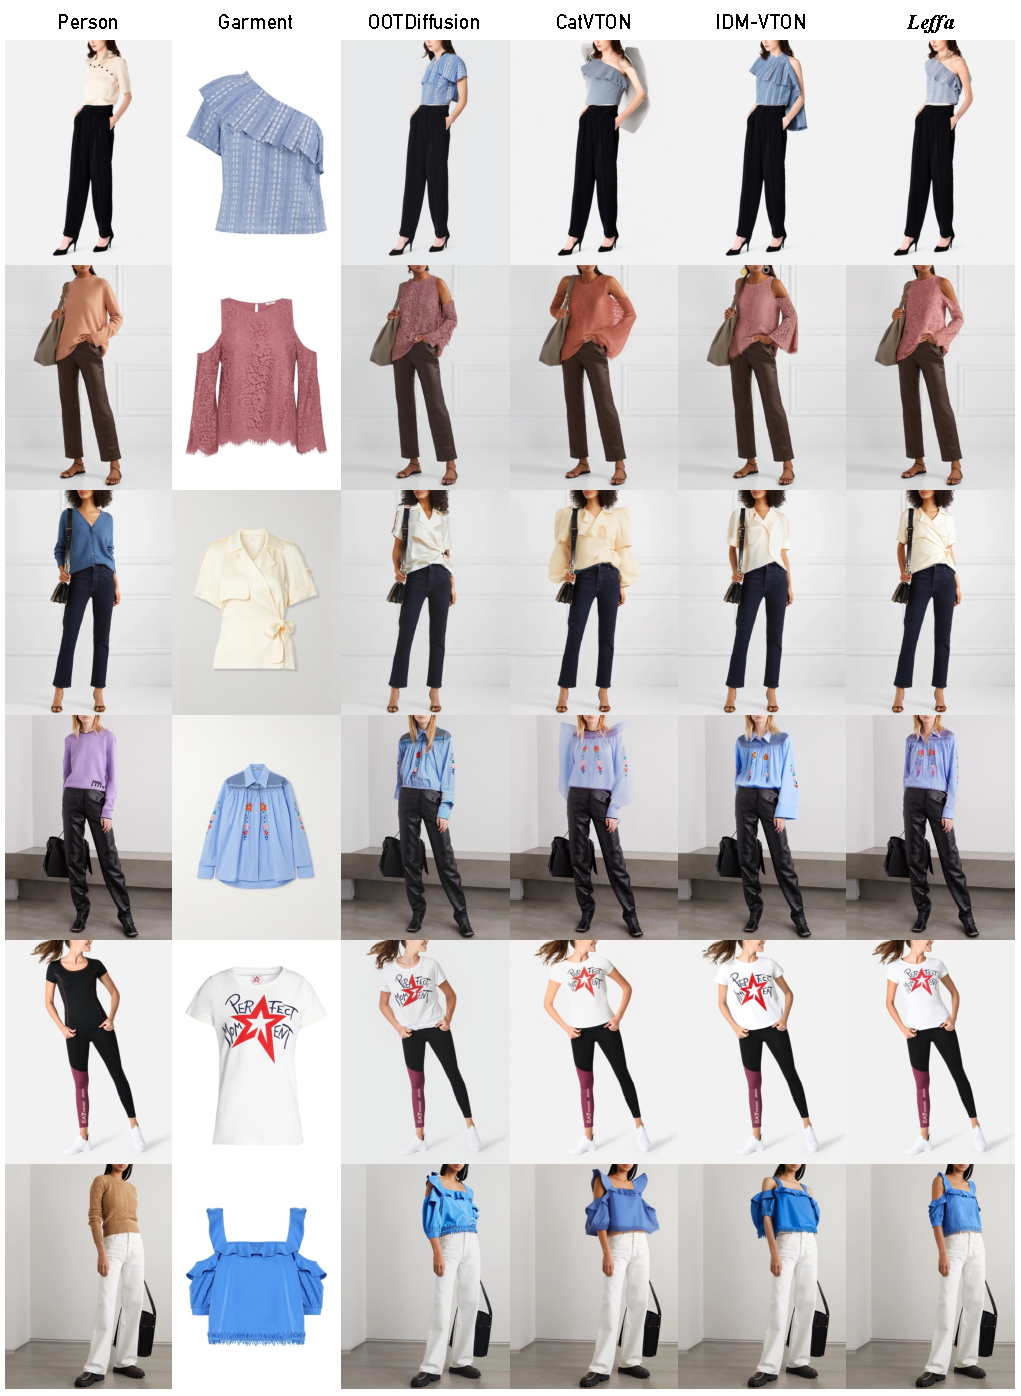
\includegraphics[width=0.95\linewidth]{Chapter6/Figures/supp_3.pdf}
%     \caption{
%     Qualitative visual results comparison with other methods on DressCode for virtual try-on (Part 1).
%     }
%     \label{leffa:fig:supp_vis_3}
% \end{figure*}

% \begin{figure*}[t]
%     \centering
%     % \fbox{\rule{0pt}{2in} \rule{1.0\linewidth}{0pt}}
%     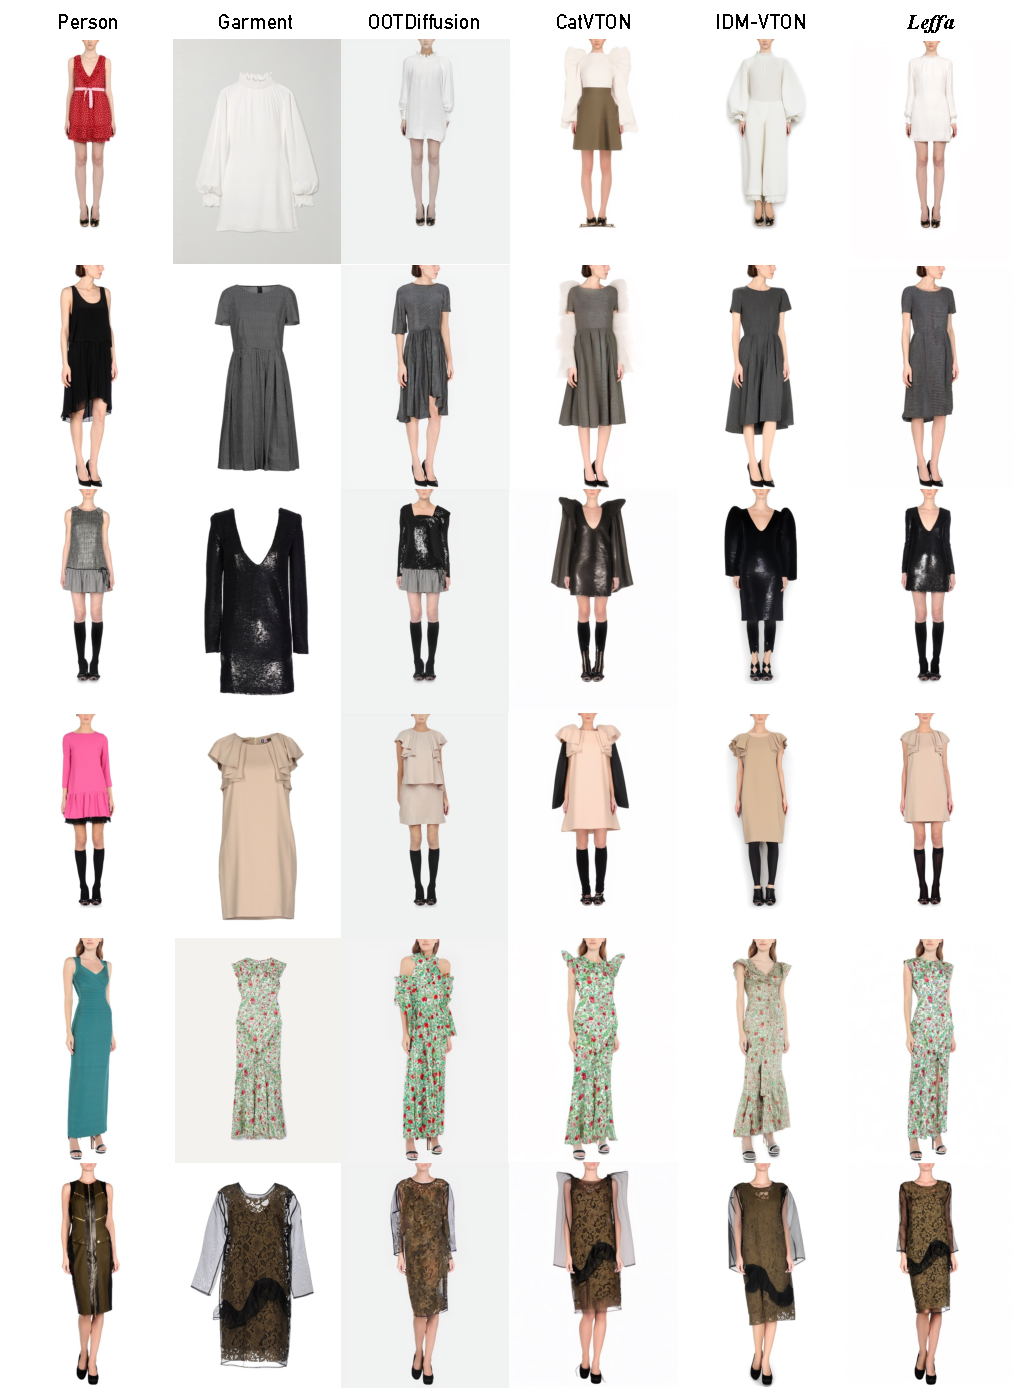
\includegraphics[width=0.95\linewidth]{Chapter6/Figures/supp_4.pdf}
%     \caption{
%     Qualitative visual results comparison with other methods on DressCode for virtual try-on (Part 2).
%     }
%     \label{leffa:fig:supp_vis_4}
% \end{figure*}

% \begin{figure*}[t]
%     \centering
%     % \fbox{\rule{0pt}{2in} \rule{1.0\linewidth}{0pt}}
%     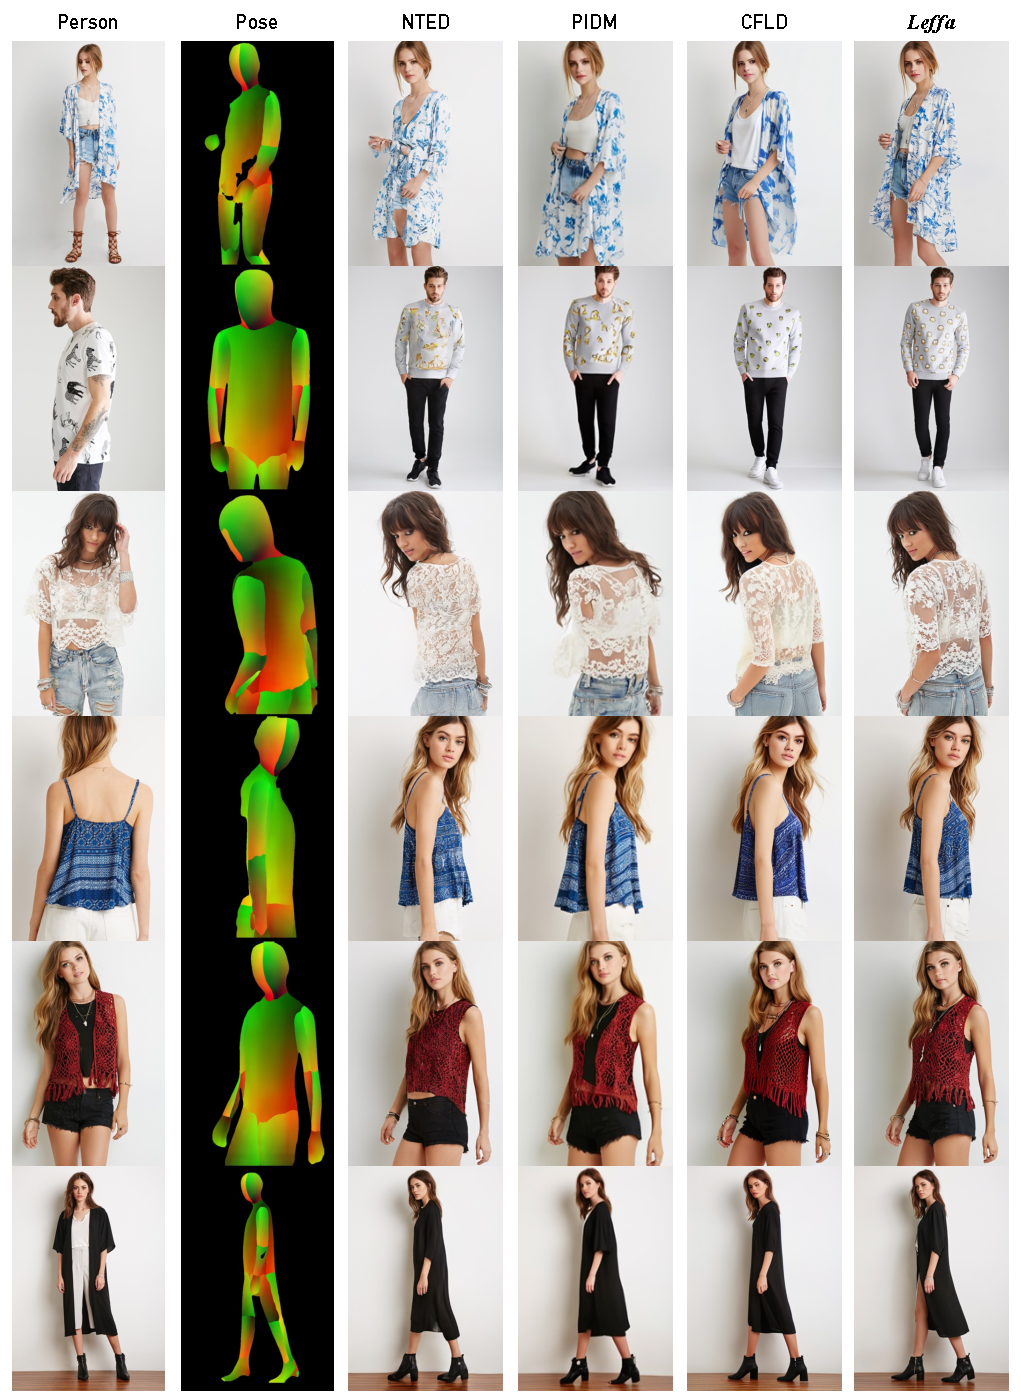
\includegraphics[width=0.95\linewidth]{Chapter6/Figures/supp_5.pdf}
%     \caption{
%     Qualitative visual results comparison with other methods on DeepFashion for pose transfer (Part 1).
%     }
%     \label{leffa:fig:supp_vis_5}
% \end{figure*}

% \begin{figure*}[t]
%     \centering
%     % \fbox{\rule{0pt}{2in} \rule{1.0\linewidth}{0pt}}
%     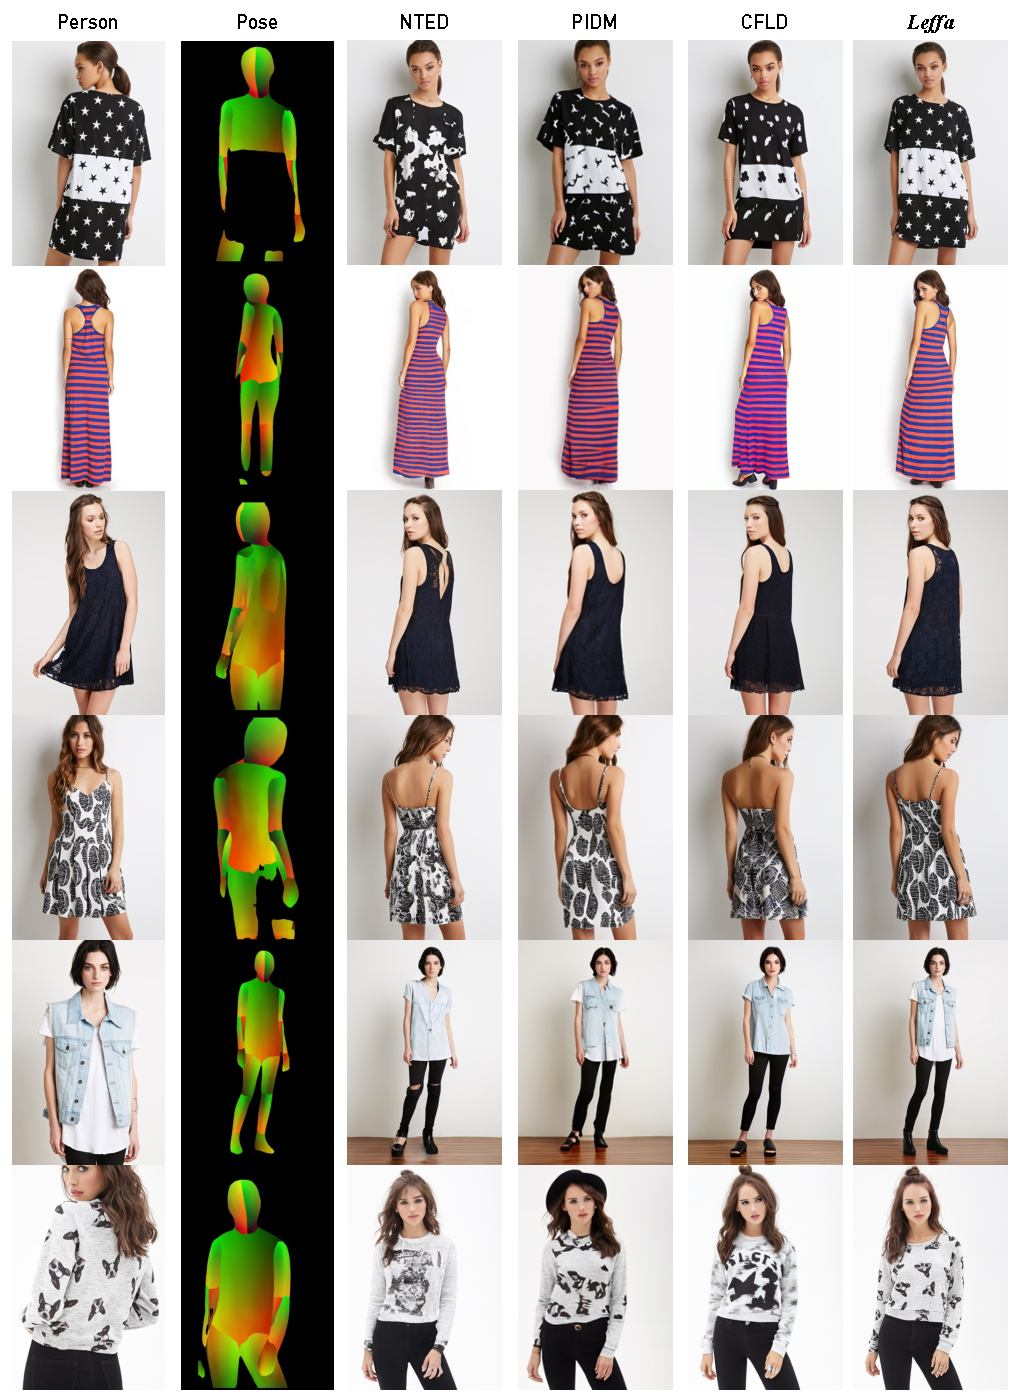
\includegraphics[width=0.95\linewidth]{Chapter6/Figures/supp_6.pdf}
%     \caption{
%     Qualitative visual results comparison with other methods on DeepFashion for pose transfer (Part 2).
%     }
%     \label{leffa:fig:supp_vis_6}
% \end{figure*}
